\documentclass{sig-alternate}
\usepackage{subfigure}
\usepackage{graphicx}
\usepackage{url}

\clubpenalty=10000
\widowpenalty = 10000


\usepackage{amsmath,amssymb}
\usepackage{amstext}
\usepackage{dsfont}
\usepackage{xspace}
\usepackage{epsfig}
\usepackage{balance}
\usepackage[noend]{algorithmic}
\usepackage{algorithm}
\usepackage{color}
\usepackage{tikz}
\usetikzlibrary{calc}


\newtheorem{conjecture}{Conjecture}
\newtheorem{mutation}{Mutation Operator}
\newtheorem{definition}{Definition}
\newtheorem{theorem}{Theorem}
\newtheorem{lemma}{Lemma}
\newtheorem{corollary}{Corollary}
\newtheorem{claim}{Claim}

\renewcommand{\epsilon}{\varepsilon}
\newcommand{\R}{\mathds{R}}
\newcommand{\N}{\mathds{N}}
\newcommand{\Q}{\mathds{Q}}
\newcommand{\Z}{\mathds{Z}}

\begin{document}

\title{ComeTogether - an android app to meet new people}

\numberofauthors{2}
\author{
	\alignauthor Christof Ochmann\\
	\affaddr{University of Applied Sciences Zittau/G\"{o}rlitz}\\
	\affaddr{02826 G\"{o}rlitz, Germany}\\
	\email{sichochm@hs-zigr.de}\\
	\and
	\alignauthor Ingo K�rner\\
	\affaddr{University of Applied Sciences Zittau/G\"{o}rlitz}\\
	\affaddr{02826 G\"{o}rlitz, Germany}\\
	\email{siinkoer@hs-zigr.de}\\
}


\maketitle
\begin{abstract}
This work based on the document "Come-Together-App", which was created in Wirtschaftsinformatik II in a course of studies of tourism. The ideas of the project "Come-Together-App"  are realized as a prototype in "ComeTogether - an android app to meet new people". Both, frontend and backend are analysed, desgined and implemented.

\end{abstract}



\category{F.2.2}{Analysis of Algorithms and Problem Complexity}{Nonnumerical Algorithms and Problems}
\terms{Algorithms, Design, Performance, Theory}
\keywords{Parallel evolutionary algorithms, island model, spatial structures, offspring populations, runtime analysis}

\input{Ingo/Introduction}

\section{requirements engineering}\label{requirementsengineering}
Figure \ref{fig:useCaseDiagram} shows the use case diagram for ComeTogether.

\section{Design}\label{Design}

In figure \ref{fig:UserServiceREST} you can see the design for the UserService. UserServiceREST encapsulate the REST-Functionality of the UserService. UserPersistence access database with prepared statements p.e. to save, read or delete users. Between UserServiceREST and UserPersistence are service class and DAO class to encapsulate different levels of abstraction. Beside UserServiceREST there are the classes EventServiceREST, ParticipationServiceREST and MessageServiceREST. EventServiceREST in figure \ref{fig:EventServiceREST} creates, reads and deletes events. ParticipationServiceREST in figure \ref{fig:ParticipationServiceREST} creates participations and gives back a list of participation for a given eventid or a given userid. MessageServiceREST in figure \ref{fig:MessageServiceREST} creates, reads or deletes messages.

\begin{figure}[htp]
\centering
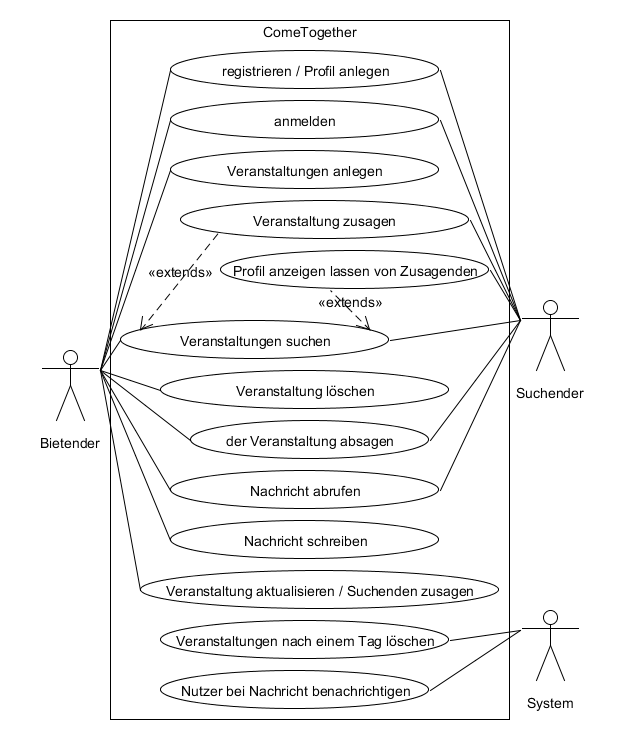
\includegraphics[width=0.5\textwidth]{Ingo/pictures/UseCaseDiagram.png}
\caption{use case diagram}
\label{fig:useCaseDiagram}
\end{figure}


\begin{figure}[htp]
\centering
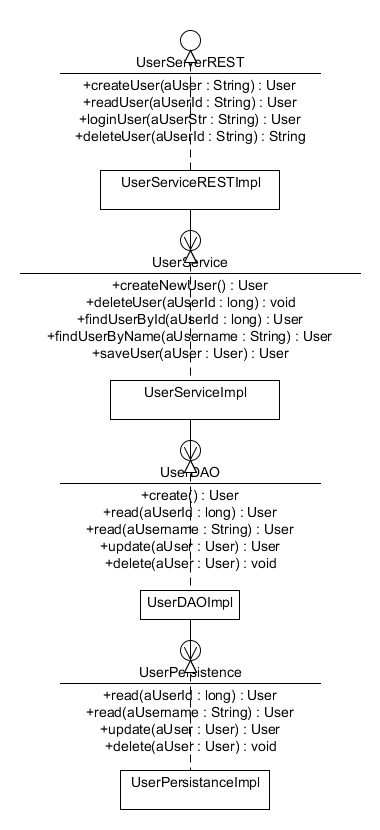
\includegraphics[width=0.5\textwidth]{Ingo/pictures/Design_User.png}
\caption{desing class diagramm UserServiceREST}
\label{fig:UserServiceREST}
\end{figure}


\begin{figure}[htp]
\centering
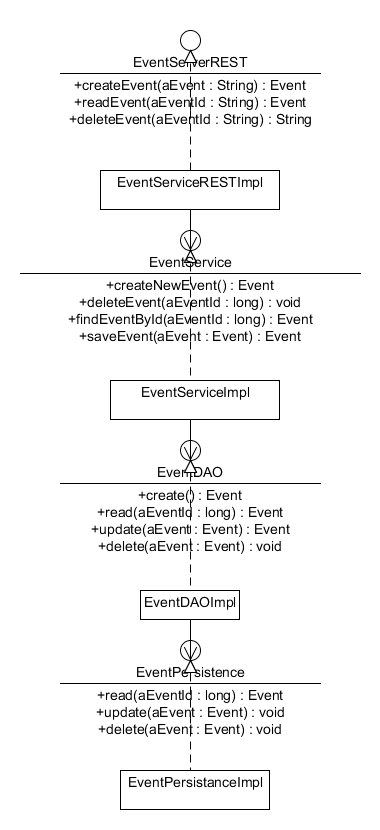
\includegraphics[width=0.5\textwidth]{Ingo/pictures/Design_Event.png}
\caption{desing class diagramm EventServiceREST}
\label{fig:EventServiceREST}
\end{figure}


\begin{figure}[htp]
\centering
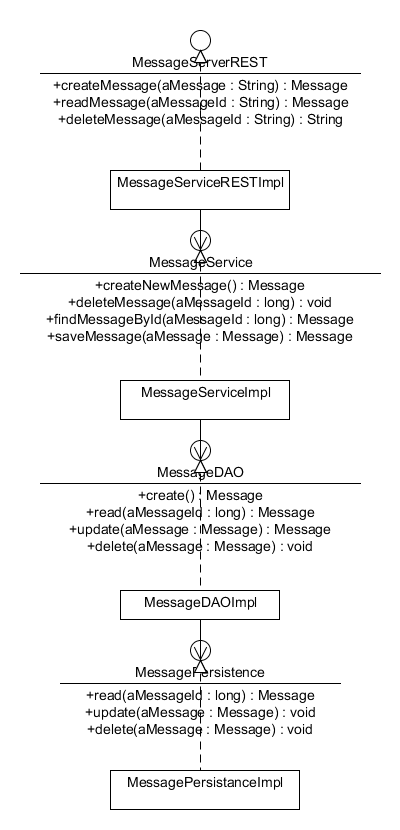
\includegraphics[width=0.5\textwidth]{Ingo/pictures/Design_Message.png}
\caption{desing class diagramm MessageServiceREST}
\label{fig:MessageServiceREST}
\end{figure}


\begin{figure}[htp]
\centering
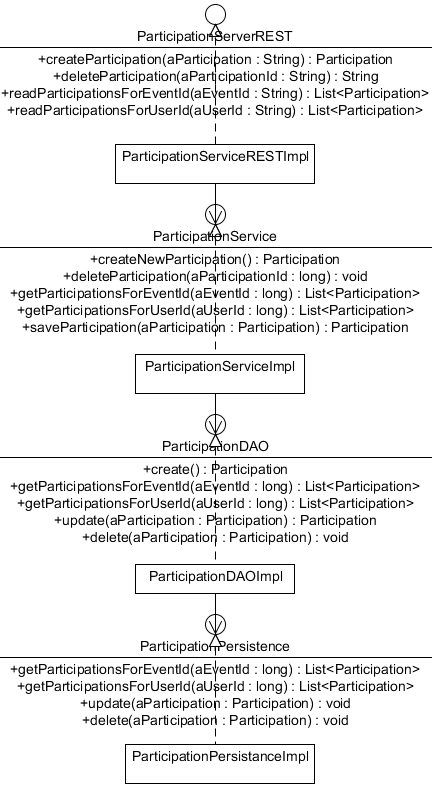
\includegraphics[width=0.5\textwidth]{Ingo/pictures/Design_Participation.png}
\caption{desing class diagramm ParticipationServiceREST}
\label{fig:ParticipationServiceREST}
\end{figure}

\section{database}\label{database}
In figure \ref{fig:EERdiagram} you can see the data base design of ComeTogether.

\begin{figure}[htp]
\centering
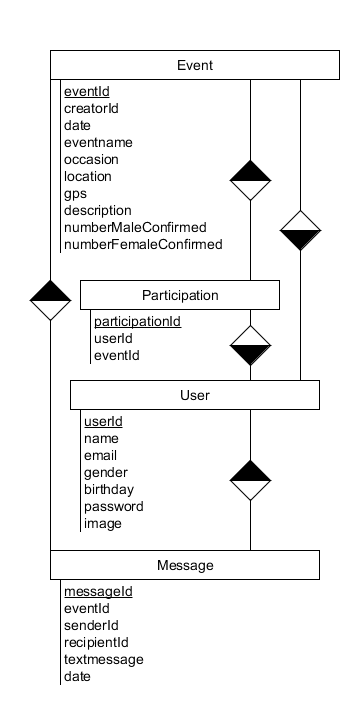
\includegraphics[width=0.5\textwidth]{Ingo/pictures/EER-diagram.png}
\caption{eer-diagram}
\label{fig:EERdiagram}
\end{figure}

%\section{User Interface Design}\label{sec:design}
Eine Webseite, wie auch eine App kommt bei den Nutzern gut an, wenn sie benutzerfreundlich und bedienbar ist. Auch wenn die Anwendung die besten und neusten Funktionen bietet, wird der User daran wenig Spa� haben, wenn er die Features nicht schnell findet oder lange navigieren muss um zu seinen gew�nschten Inhalten zu gelangen. Schon in den 90er Jahren hat sich Jakob Nielsen, ein d�nischer Schriftsteller und mittlerweile eine der f�hrenden Pers�nlichkeiten auf dem Gebiet der Benutzerfreundlichkeit, ausf�hrlich mit dem Themen Webdesign und Usability besch�ftigt. In diesem Zusammenhang erstellte er eine Liste mit zehn Grundprinzipien, die man bei der Gestaltung von Bedienoberfl�chen beachten sollte. Die Grundprinzipien wurden mit dem Gedanken an die Gestaltung von Webseiten erstellt, gelten aber zum Teil genauso f�r Apps. \\  %hier link%
\subsection{Design einer Android-App}
Auf der Google I/O 2010 pr�sentierte Jim Palmer das erste Mal Richtlinien, an die man sich halten kann bei der Entwicklung von Android-Apps. Sie beschreiben wie eine App auszusehen hat:
\begin{itemize}
\item einfach und verst�ndlich
\item sich auf den Inhalt konzentrieren und nicht nur auf das Aussehen
\item konsistent sein, damit sich der Nutzer schnell zurechtfinden kann
\end{itemize}
Bei der Entwicklung der ComeTogether-App war es uns wichtig sich an diese Guidelines zu halten und somit mussten die uns zur Verf�gung stehenden GUI-MockUps der zu entwickelnden App angepasst werden, bevor wir mit der Umsetzung des Frontends beginnen konnten. Daf�r benutzen wir das Tool Balsamiq Mockups. Per Drag \& Drop lassen sich ganz einfach GUI-Element(Formularfelder, Navigationsleisten, Tabs usw.) auf einer Arbeitsfl�che zusammenklicken. Auf der Webseite mockupstogo gibt es f�r Android oder iOS Erweiterungen falls die Standardelemente nicht ausreichen. 
\subsection{Sherlock ActionBar}
Ab Android 3.0(Honeycomb) ersetzt die Action Bar das Options-Men�(als Popup-Men� mit der Men�-Taste aufrufbar) sowie die Title Bar. Die Action Bar erlaubt Menus und Buttons zu platzieren und bietet die M�glichkeit sich in einen oberen und einen unteren Teil aufzuteilen. Die Action Bar ist immer am Screen sichtbar(kann mit hide() unsichtbar gemacht werden) und macht somit das User Interface konsistent, was viel dazu beitr�gt das Design der App benutzerfreundlich zu gestalten. \\
Um die Action Bar auf Android 2.x nutzen zu k�nnen wurde die Open-Source-Library ActionBarSherlock entwickelt. Dabei handelt es sich um eine Erweiterung der Support Library, die es erm�glicht APIs auf �lteren Android-Platformen zu nutzen. %hier link zu support library  http://developer.android.com/tools/extras/support-library.html% 
Mit der neusten Version der ActionBarSherlock(v4.1.0) soll es dem App-Entwickler m�glich sein, die Action Bar aus Android 4.0(Ice Cream Sandwich) mit allen Features auf 2.x nutzbar zu machen. Auf der Projektseite von ActionBarSherlock gibt es einige Demos, sowie einen Link zur GitHub-Seite mit allen Quellcodes. Um ein Android-Projekt mit der ActionBarSherlock aufsetzen zu k�nnen geht man wie folgt vor:
\begin{enumerate}
\item Nachdem man ActionBarSherlock heruntergeladen hat, findet man einen Ordner "`library"', den man als "`new Android project - from existing source"' in Eclipse importieren muss. In diesem Projekt klickt man unter Properties/Android das H�kchen bei "`Is library"' an.
\item Im eigentlichen Android-Projekt geht man in Properties/Android und klickt auf add. Daraufhin sollte die ABS-library erscheinen und in das Projekt eingebunden werden k�nnen.
\item In der AndroidManifest.xml muss f�r jede activity, die die ABS haben soll, der style festgelegt werden mit der folgenden Zeile: \\
 android:theme="'@style/Theme.Sherlock.Light"'> 
 \item In dem activities wird die ABS mit extends vererbt und mit der folgenden Methode aufgerufen: \\
 \begin{verbatim}
 public boolean onCreateOptionsMenu(Menu menu) {
    ...
    } 
 \end{verbatim}
\end{enumerate}

\subsection{Hintergrundoperationen}
\subsubsection{REST-Kommunikation}
Um auf die Methoden des RESTful-Webservice zugreifen zu k�nnen werden zuerst die Instanzen von dem jeweiligen Datentyp wie beispielsweise User mit allen notwendigen Daten bef�llt, %hier auf listing verweisen
anschlie�end wird eine Instanz des UserClient erstellt und deren Methode createUser(user) aufgerufen. Die Methode createUser erbt von der abstrakten Klasse Creator und initialisiert eine Verbindung zum Webservice mit initConnection("`http://10.0.2.2:8080/ctBackend/ctUser/createUser"') um anschlie�end die Methode writeProduct aufzurufen, die schlie�lich post.setEntity(new StringEntity(product)) ausf�hrt und die Daten an den Server per POST sendet.
\subsubsection{UI-Thread und langlaufende Programmteile}
UI-Thread ist in einer Android-App f�r die Darstellung und Anwendereingaben zust�ndig. Alle Methoden einer Android-Komponente, die mit "`on"' beginnen, wie z.B. onClick laufen in diesem UI-Thread und d�rfen nicht blockieren, das bedeutet, dass alle Methoden, die auf Oberfl�chenereignisse reagieren, schnell abgearbeitet werden m�ssen(innerhalb f�nf Min.). Werden sie nicht innerhalb dieser Zeitspanne abgearbeitet, und der Nutzer dr�ckt z.B. auf die Men�taste, dann geht Android davon aus, dass die Anwendung abgest�rzt ist und der Nutzer bekommt einen Application not responding(ANR) angezeigt. Eine L�sung hierf�r w�re ein eigener Thread, der in dieser onClick-Methode ausgef�hrt wird, damit die Anwendung m�glichst schnell auf Nutzereingaben reagiert und nicht blockiert. Das Problem dabei ist, dass die Anzeige nur der UI-Thread ver�ndern darf und jeder Zugriff von au�erhalb zu einer Exception f�hrt. Man br�uchte noch eine zus�tzlichen Thread, der mit Hilfe eines Handlers eine Nachricht dem UI-Thread �bergibt und dieser die Informationen aus dem ersten Thread holt und anzeigt. Denn es ist anderen Threads nicht erlaubt, Daten im UI-Thread zu ver�ndern, da eine Ver�nderung des UI-Threads die Synchronisierung der Objektzust�nde erforderlich machen w�rde und somit nicht automatisch ausgef�hrt wird. Das ganze ist mit Threads sehr kompliziert und wird in Android auf eine einfachere Art und Weise mit Hilfe von AsyncTask gel�st.
\subsection{AsyncTask}
AsyncTask ist eine Klasse, die es erm�glicht Operationen im Hintergrund zu bearbeiten und anschlie�end einen Code im UI-Thread auszuf�hren. Um die Klasse zu nutzen muss man eine Unterklasse von AsyncTask erstellen. AsyncTask enth�lt drei Methoden, die in der Unterklasse �berschrieben werden m�ssen:
\begin{itemize}
\item doInBackground(): \\
Hier steht der Code, der im Hintergrund, in einem separaten Thread, ausgef�hrt werden soll. Beim Aufruf mit execute() kann der Methode als Parameter ein String �bergeben werden, der dann in der eigentlichen Methode in ein String-Array umgewandelt wird.
\item onProgressUpdate(): \\
Dieser Code-Abschnitt wird ausgef�hrt, wenn es einen Fortschritt bei der Ausf�hrung gibt, der aus der doInBackground-Methode gemeldet wird. Der Fortschritt kann beispielsweise der prozentuale Anteil einer heruntergeladenen Datei sein. 
\item onPostExecute(): \\
Diese Methode wird aufgerufen, wenn die doInBackground-Methode abgearbeitet ist. Es handelt sich um die Benutzerschnittstelle, die dem Nutzer meldet, dass die Aufgabe erledigt worden ist. Das Argument dieses Methodenaufrufs ist der Parameter, den die doInBackground-Methode zur�ckliefert.
\end{itemize}
Um den AsyncTask auszuf�hren wir die Unterklasse instantiiert und die Methode execute() aufgerufen. Die Frage ist nun wann man AsyncTask einsetzen sollte. Ab besten ist es so viel wie m�glich in den Hintergrund zu verschieben, denn der UI-Thread f�hrt nur �nderungen an der Anzeige aus, wenn er nicht besch�ftigt ist. Deswegen sollten Aufrufe, die etwas l�ngern dauern, wie beispielsweise der Datenbankzugriff, ein Webservice-Aufruf, das Parsen eines JSON-Objekts usw. in einem AsyncTask aufgerufen werden. Mit einem Ladebalken kann dem Nutzer mitgeteilt werden wie der Fortschritt der Aufgabe ist und ihm dadurch das Gef�hl vermitteln, dass die App schnell und fl�ssig l�uft. Mit der Methode isFinishing() kann in onPostExecute() gepr�ft werden, ob die Activity, in der der AsyncTask l�uft nicht mittlerweile beendet worden ist, weil es kann vorkommen, dass der Nutzer die Activity geschlossen hat, aber der AsyncTask noch l�uft und versuchen wird die onPostExecute() auszuf�hren. \\
In der ComeTogether-App nutzen wir die Vorteile der AsyncTask u.a. bei Zugriffen auf den Webservice.

\subsection{�bergabe von Objekten zwischen Activities}
Nachdem ein User auf ComeTogether sich erfolgreich eingeloggt hat, liefert der Webservice ein Objekt der Klasse User. Dieses Objekt muss zwischen Activities �bertragen werden und jederzeit zur Verf�gung stehen.
\begin{enumerate}
\item Interface Parcelable implementieren:\\ Damit die Instanzen der Klasse User zwischen Activities ausgetauscht werden k�nnen, muss die Klasse User das Interface Parcelable implementieren. Anschlie�end kann man ganz einfach mit einem Intent die Objekte an die andere Activity weiterreichen, z.B. intent.putExtra("`user"', new User()); Die Daten bokommt man aus dem Bundle folgenderma�en: Bundle data = getIntent().getExtras(); User user = data.getParcelable("`user"');
\item Objekt serializieren:\\ Eine weitere, aber weniger ressourcenschonende M�glichkeit bietet java.io.Serializable. Die Klasse User m�sste das Interface Serializable implementieren. Anschlie�end braucht man einen neuen Intent und Bundle. Mit der putSerializable("`user"', new User()) wird das Objekt dem Bundle hinzugef�gt und mit intent.putExtras(bundle) das Bundle an das Intent angeh�ngt. Mit startActivity(intent) wird die n�chste Activity gestartet und das Objekt kann mit User user = (User)getIntent().getSerializableExtra("`user"') geholt werden.  
\item In der SQLite Datenbank speichern:\\ Als beste und einfachste M�glichkeit das User-Objekt allen notwendigen Activities jederzeit verf�gbar zu machen erwie� sich die Speicherung der User-Daten intern in der SQLite Datenbank.  
\end{enumerate}






    





\section{Preliminaries}
\label{sec:Preliminaries}

\section{Previous Work}
\label{sec:PreviousWork}


\section{Sorting}
\label{sec:Sorting}

...


\section{Shortest Paths}
\label{sec:ShortestPaths}


...


\section{Eulerian Cycles}
\label{sec:EulerianCycles}

...

\subsection{Edge Walks}

...

\subsection{Restricted Mutation Operators}

...

\subsection{Adjacency List Matchings}

...

\section{Conclusions}
\label{sec:Conclusions}


\subsection*{Acknowledgments}
The authors would like to thank .....the German fast food industry for keeping us alive.

\bibliographystyle{abbrv}
\bibliography{literature-short}
\balance

\end{document}
